\documentclass[12pt,a4paper]{article}

\usepackage[utf8]{inputenc}
\usepackage[T1]{fontenc}
\usepackage{lmodern}
\usepackage{geometry}
\usepackage{amsmath}
\usepackage{amssymb}
\usepackage{booktabs}
\usepackage{longtable}
\usepackage{array}
\usepackage{hyperref}
\usepackage{xcolor}
\usepackage{listings}
\usepackage{enumitem}
\usepackage{graphicx}
\usepackage{pdflscape}

\geometry{margin=1in}
\emergencystretch=1.5em
\hypersetup{
    colorlinks=true,
    linkcolor=blue,
    urlcolor=blue,
    citecolor=blue
}

\lstset{
    basicstyle=\ttfamily\small,
    frame=single,
    breaklines=true,
    showstringspaces=false
}

\title{\textbf{PF / SSSA / TS Technical Report}\\
\large In-House Power-System Stability Toolkit --- Equation-Audited}
\author{Technical Report}
\date{\today}

\begin{document}

\maketitle

\begin{abstract}
This report documents the AC power flow (PF), small-signal stability analysis
(SSSA), and transient stability simulation (TS) capabilities of the in-house
MATLAB power-system stability toolkit. It covers three synchronous-generator
models (classical second-order, Padiyar model-1.1, operational EMF6), the
implicit trapezoidal integration method, and both fixed-step and adaptive-step
time integration with step-doubling local-truncation-error estimation. Results
are validated against PSAT and PGAz for the IEEE 14-bus and IEEE RTS-24 systems,
and against the Padiyar four-machine two-area textbook case. Every equation
carries a provenance chain from source to implementation; every table and
figure is emitted by a tracked MATLAB command (\texttt{generate\_system\_methods\_report})
against a clean committed HEAD. No computed value is typed manually. Results
are generated fresh; the equation provenance audit gate is READY.
\end{abstract}

\section{Title, abstract and reproducibility statement}

\paragraph{Scope.} This report covers PF, SSSA, TS, synchronous-generator
models, and fixed/adaptive integration for three study cases: IEEE 14-bus
(primary, per advisor directive 2026-07-12), IEEE RTS-24, and the Padiyar
four-machine two-area system.

\paragraph{Selected Git revision.} Results were generated against
\texttt{REPORT\_HEAD} (the \texttt{report/system-methods-v2} branch HEAD),
a clean committed HEAD where the production default stepper is \texttt{fixed}.
The dirty \texttt{run\_ts.m} edit on \texttt{main} is excluded user work and
was not carried into the report worktree.

\paragraph{No predeclared PASS.} Validation status is reported per-case with
numeric metrics; no unqualified PASS is declared. PSAT/PGAz are validation
references only and never enter the production solver path.

\section{Nomenclature and conventions}

\paragraph{Bases.} $S_{\mathrm{base}}$ (three-phase MVA), $V_{\mathrm{base}}$
(line-to-line kV), $f$ (Hz). Per-unit on the three-phase system base.
$Z_{\mathrm{base}}=V_{\mathrm{base}}^2/S_{\mathrm{base}}$,
$I_{\mathrm{base}}=S_{\mathrm{base}}/V_{\mathrm{base}}$ (line-to-line /
three-phase factors implicit in $S_{\mathrm{base}}$).

\paragraph{Bus and generator indexing.} External bus IDs from case data;
internal bus types $1{=}\text{REF}$, $2{=}\text{PV}$, $3{=}\text{PQ}$ (MATPOWER:
$3{=}\text{REF}$, $2{=}\text{PV}$, $1{=}\text{PQ}$).

\paragraph{Complex voltage.} $V_i=|V_i|e^{j\theta_i}$. Current direction:
positive from generator into network. Generator injection sign: positive
$P,Q$ means injection into the bus. Complex power $S_i=P_i+jQ_i=V_i I_i^*$
(PF-07).

\paragraph{Rotor angle reference.} Electrical radians relative to the slack
bus angle. Speed in pu (absolute, $1$ at synchronous) and rad/s
($\omega_b=2\pi f$).

\paragraph{COI angle.} $\delta_{\mathrm{COI}}=\sum_i H_i\delta_i/\sum_i H_i$
(inertia-weighted). COI-relative and incremental angle metrics remove
common-mode motion (CMP-04/05).

\paragraph{DAE.} Differential state $x$, algebraic state $y$ (interleaved
$[\mathrm{Re}(V_1),\mathrm{Im}(V_1),\ldots]$), input $u$. Network residual
$g(x,y,u)=0$.

\paragraph{KCL residual sign (traced from code).} The production network
residual is current balance $g = I_{\mathrm{inj}} - Y_{\mathrm{bus}}V = 0$
(\texttt{synchronous\_emf6\_ssa.m:168--169}: $\mathrm{Inet}{=}Y V$;
$g{=}{-}\mathrm{Inet}$ then generator currents added). For the classical
linear network, $V=(Y{+}Y_{\mathrm{gen}})\backslash I_{\mathrm{inj}}$
(\texttt{classical\_dae.m:139}). Injection is positive into the bus.

\paragraph{Units.} Voltage pu, angle deg (plots) / rad (equations), power pu
or MW ($\times S_{\mathrm{base}}$), frequency Hz, damping ratio dimensionless,
eigenvalues $s^{-1}$.

\section{Case and provenance matrix}

\begin{longtable}{p{2.8cm}p{2.2cm}p{2.2cm}p{2cm}ccccp{1.8cm}}
\toprule
Case & Network source & Dynamic source & Reference & PF & SSSA & TS & Ours/PSAT/PGAz & Freshness \\
\midrule
IEEE 14-bus & MATPOWER 6 & ASSUMED\_DIAGNOSTIC & PSAT+PGAz & \checkmark & \checkmark & \checkmark & Ours/PSAT/PGAz & fresh \\
IEEE RTS-24 & RTS-96 & RTS-96 & PSAT & \checkmark & \checkmark & \checkmark & Ours/PSAT & fresh \\
Padiyar 4M2A & Padiyar Tab.9.1 & Padiyar model-1.1 & Padiyar Tab.9.2/9.5 & \checkmark & \checkmark & \checkmark & Ours/book & fresh \\
Kundur 4M2A & \multicolumn{8}{l}{Not used in this report (legacy calibrated GENTPJ excluded per AGENTS.md).} \\
\bottomrule
\end{longtable}

\paragraph{No conflation.} Padiyar and Kundur four-machine two-area systems
are never treated as reproductions of each other.

\section{AC power-flow formulation}

The production PF solver is \texttt{pfsolver.powerflow\_newton\_raphson}
(in-house Newton--Raphson, no external nonlinear solver). External tools
(PSAT/PGAz/MATPOWER) are references only.

\paragraph{PF-01 per-unit bases.}
$Z_{\mathrm{base}}=V_{\mathrm{base}}^2/S_{\mathrm{base}}$,
$I_{\mathrm{base}}=S_{\mathrm{base}}/V_{\mathrm{base}}$.
Line-to-line/three-phase factors implicit in $S_{\mathrm{base}}$.

\paragraph{PF-02 series branch admittance.}
$y_{ik}=1/(r_{ik}+jx_{ik})$.

\paragraph{PF-03 transformer tap/phase-shift.}
Off-nominal tap $a=t\,e^{j\phi}$:
$Y_{ii}\mathrel{+}=y/(a\overline{a})+jb/2$,
$Y_{ij}\mathrel{-}=y/\overline{a}$,
$Y_{ji}\mathrel{-}=y/a$,
$Y_{jj}\mathrel{+}=y+jb/2$
(\texttt{classical\_dae.m:229--233}).

\paragraph{PF-04 shunt and line-charging.}
$Y_{ii}\mathrel{+}=G_{\mathrm{sh}}+jB_{\mathrm{sh}}$; half-line charging
$jb/2$ at each end.

\paragraph{PF-05 Ybus assembly.}
Diagonal accumulates branch admittances, shunts, charging; off-diagonal is
$-y$ (or $-y/\overline{a}$ for tap). Hermitian structure for non-phase-shifting
branches.

\paragraph{PF-06 network current equation.}
$I=Y_{\mathrm{bus}}V$. Classical: $V=(Y{+}Y_{\mathrm{gen}})\backslash I_{\mathrm{inj}}$.

\paragraph{PF-07 complex power convention.}
$S_i=P_i+jQ_i=V_i I_i^*$. Verified: $P_e=\mathrm{Re}(V\overline{I_g})$
(\texttt{classical\_dae.m:145}).

\paragraph{PF-08/09 expanded injections.}
$P_i=\sum_k |V_i||V_k|(G_{ik}\cos\theta_{ik}+B_{ik}\sin\theta_{ik})$;
$Q_i=\sum_k |V_i||V_k|(G_{ik}\sin\theta_{ik}-B_{ik}\cos\theta_{ik})$.

\paragraph{PF-10 scheduled net injection.}
$P_i^{\mathrm{spec}}=P_{G,i}-P_{L,i}$, $Q_i^{\mathrm{spec}}=Q_{G,i}-Q_{L,i}$.

\paragraph{PF-11 mismatch.}
$\text{mismatch}=[P^{\mathrm{spec}}-P^{\mathrm{calc}};\;Q^{\mathrm{spec}}-Q^{\mathrm{calc}}]$.

\paragraph{PF-12 Newton linearization.}
$J[\Delta\theta;\Delta|V|]=[\Delta P;\Delta Q]$. Backslash, no inverse
(\texttt{powerflow\_newton\_raphson.m:212}).

\paragraph{PF-13 four Jacobian blocks.}
$H=\partial P/\partial\theta$, $N=\partial P/\partial|V|$,
$M=\partial Q/\partial\theta$, $L=\partial Q/\partial|V|$.

\paragraph{PF-14 state update and stopping.}
$x\mathrel{+}=\Delta x$; stop when $\max|\text{mismatch}|<\text{tol}$ (default
$10^{-6}$, PF uses $10^{-10}$).

\paragraph{PF-15 PV-to-PQ switching.}
If $Q_g$ violates $Q_{\min}/Q_{\max}$, fix $Q$ at the limit and switch PV to PQ
(\texttt{find\_q\_limit\_violations}).

\paragraph{PF-16 slack recovery.} REF bus $P,Q$ recovered from solved $V$.

\paragraph{PF-17 branch flows.}
$I_{ij}=y_{ij}(V_i-V_j)+jb/2\,V_i$; $S_{ij}=V_i\overline{I_{ij}}$.

\paragraph{PF-18 losses.}
$P_{\mathrm{loss}}=\sum\mathrm{Re}(S_{ij}+S_{ji})$.

\paragraph{PF-19 power-balance residual.}
$P_{\mathrm{gen}}=P_{\mathrm{load}}+P_{\mathrm{loss}}$ at convergence.

\section{Synchronous-generator models}

Three distinct models, never merged.

\subsection{Classical second-order model}

States $x=[\delta;\omega]$ per machine; $E=|E|e^{j\delta}$ constant behind
$X'_d$.
\begin{align}
\dot\delta_i &= \omega_b(\omega_i-1) \\
\dot\omega_i &= \frac{P_{m,i}-P_{e,i}-D_i(\omega_i-1)}{2H_i}
\end{align}
Verified verbatim at \texttt{classical\_dae.m:116}: \texttt{dx=[ws*(w-1); (Pm-Pe-D*(w-1))./(2*H)]}. Denominator is $2H$ (not $H$); $\omega_b=2\pi f$.
$E=V+jX'_d I$ (\texttt{classical\_dae.m:60}); $I_g=(E-V)/(jX'_d)$;
$P_e=\mathrm{Re}(V\overline{I_g})$.

\subsection{Padiyar model-1.1 (four-machine two-area)}

States per machine (AVR): $[\delta,\omega,E'_q,E'_d,E_{fd}]$ (manual: 4 states).
\begin{align}
\dot\delta &= \omega_B(\omega-1) \\
\dot\omega &= \frac{P_m-P_e-D(\omega-1)}{2H} \\
\dot E'_q &= \frac{E_{fd}-E'_q-(X_d-X'_d)I_d}{T'_{d0}} \\
\dot E'_d &= \frac{-E'_d+(X_q-X'_q)I_q}{T'_{q0}} \\
\dot E_{fd} &= \frac{K_A(V_{\mathrm{ref}}-|V_t|)-E_{fd}}{T_A}
\end{align}
Verified at \texttt{padiyar\_model11\_dae.m:128--133}. Source: Padiyar,
\emph{Power System Dynamics}, 2nd ed., Section 9.6.1, Tables 9.1--9.5
(printed pp.~325--331). $V_{\mathrm{ref}}=|V_t|+E_{fd}/K_A$ at initialization.

\subsection{Operational EMF6 model}

States per machine: $[\delta,\omega,E'_q,E'_d,E''_q,E''_d]$ (six states).
\begin{align}
\dot\delta &= \omega_0\omega \\
\dot\omega &= \frac{T_m-T_e-D\omega}{2H} \\
\dot E'_q &= \frac{E_{fd}+c_d E''_q-d_d E'_q}{T'_{d0}} \\
\dot E'_d &= \frac{c_q E''_d-d_q E'_d}{T'_{q0}} \\
\dot E''_q &= \frac{E'_q-E''_q-(X'_d-X''_d)I_d}{T''_{d0}} \\
\dot E''_d &= \frac{E'_d-E''_d+(X'_q-X''_q)I_q}{T''_{q0}}
\end{align}
Verified at \texttt{synchronous\_emf6\_ssa.m:158--163}. Air-gap torque
$T_e=V_d I_d+V_q I_q+R_a(I_d^2+I_q^2)$ (\texttt{synchronous\_emf6\_ssa.m:157}).
Legacy calibrated GENTPJ and primitive-flux paths are in \texttt{legacy/},
off the path, and are NOT production equations.

\section{SSSA methodology}

Start from the DAE $\dot x=f(x,y,u)$, $0=g(x,y,u)$. At equilibrium
$f(x_0,y_0,u_0)=0$, $g(x_0,y_0,u_0)=0$. First-order Taylor expansion gives the
four Jacobian blocks $J_{xx},J_{xy},J_{yx},J_{yy}$ (central finite differences,
\texttt{synchronous\_emf6\_ssa.m:216--227}, $h=3\times10^{-6}$).
\begin{equation}
\begin{bmatrix}\Delta\dot x\\0\end{bmatrix}=
\begin{bmatrix}J_{xx}&J_{xy}\\J_{yx}&J_{yy}\end{bmatrix}
\begin{bmatrix}\Delta x\\\Delta y\end{bmatrix}
\end{equation}
Eliminate $\Delta y$ via backslash (never inverse):
\begin{equation}
A=J_{xx}-J_{xy}(J_{yy}\backslash J_{yx})
\end{equation}
(\texttt{multimachine\_ssa.m:44}; \texttt{free\_y} selects retained
algebraic variables, default $1{:}n_y$.) Eigenvalues
$\lambda_i=\sigma_i+j\omega_i$; frequency $f_i=|\omega_i|/(2\pi)$; damping ratio
$\zeta_i=-\sigma_i/|\lambda_i|$ (\texttt{multimachine\_ssa.m:67--68}).
Stability: all $\mathrm{Re}(\lambda)<-10^{-9}$; zero eigenvalues are reference
modes (removed by optional COI reduction). Eigenvalue pairing between Ours and
references uses a deterministic greedy assignment (no manual pairing).

\section{TS numerical method}

Implicit trapezoidal update:
\begin{equation}
x_{n+1}=x_n+\frac{h}{2}\bigl[f(t_n,x_n,y_n)+f(t_{n+1},x_{n+1},y_{n+1})\bigr]
\end{equation}
with algebraic constraint $g(t_{n+1},x_{n+1},y_{n+1})=0$
(\texttt{ts\_step\_kernel.m:78,163}).
Corrector residual $R_x=x_{n+1}-x_n-\frac{h}{2}(f_n+f_{n+1})$
(\texttt{ts\_step\_kernel.m:82,165}); algebraic residual
$R_g=g(t_{n+1},x_{n+1},y_{n+1})$. The corrector iterates until both the
state update and the trapezoidal residual are below tolerance.

\paragraph{Event convention.} Event times are snapped to the grid
(\texttt{ts\_adaptive\_driver.m:92--100}). The arrival step uses the LEFT
topology; at the event, the topology switches to RIGHT and the algebraic
variables are re-solved under the new topology
(\texttt{ts\_adaptive\_driver.m:160--185}). No trapezoidal step spans two
topologies. The public sample uses the RIGHT-limit voltage (faulted).

\section{Fixed-step and adaptive-step methods}

\subsection{Fixed time step}

$h$ is fixed except for exact event landing. The corrector iteration count is
\emph{fixed} for EMF6 (default \texttt{corrector\_iter=3},
\texttt{ts\_simulate\_emf6}) and \emph{residual-controlled} (adaptive) for the
classical and Padiyar paths. ``Adaptive corrector'' (variable iteration count
at fixed $h$) is distinct from ``adaptive time step'' (variable $h$ with LTE
rejection); the two are never conflated.

\subsection{Adaptive time step}

\paragraph{Layer 1 --- continuous problem.}
$\dot x=f(t,x,y,u)$, $0=g(t,x,y,u)$. $x$: differential states (rotor angle,
speed); $y$: algebraic (bus voltages); $u$: mechanical/excitation inputs.
Smooth between discrete network events; fault application and clearing divide
the trajectory into topology segments.

\paragraph{Layer 2 --- base integration.}
Trapezoidal quadrature $\int_t^{t+h}f\,d\tau=\frac{h}{2}[f(t)+f(t+h)]+O(h^3)$
gives the update above with $R_x$ and $R_g$ (RUNTIME\_EQUATION). Implicit:
$f_{n+1}$ depends on the unknown $x_{n+1},y_{n+1}$.

\paragraph{Layer 3 --- accuracy theory and step doubling.}
Method order $p=2$ (local error $O(h^3)$, global $O(h^2)$). Full step:
$x_h=x^\ast+Ch^{p+1}+O(h^{p+2})$. Two half steps:
$x_{h/2,h/2}=x^\ast+2C(h/2)^{p+1}+O(h^{p+2})=x^\ast+2^{-p}Ch^{p+1}+O(h^{p+2})$.
Subtract: $x_{h/2,h/2}-x_h=(2^{-p}-1)Ch^{p+1}+O(h^{p+2})$.
The fine-solution estimator (project-derived, proven by
\texttt{test\_ts\_adaptive\_lte} Test C; Hairer section/page unverified on
this host per \texttt{adaptive\_ts\_track\_a.md}):
\begin{equation}
e_{\mathrm{fine}}\approx\frac{x_{h/2,h/2}-x_h}{2^p-1}=\frac{x_{h/2,h/2}-x_h}{3}
\quad(p=2)
\end{equation}
The project accepts the fine solution $x_{h/2,h/2}$
(\texttt{ts\_adaptive\_driver.m:153}). The full step $x_h$ is used only to
form the estimate.

\paragraph{Layer 4 --- runtime adaptive controller.}
Scaling $s_{x,i}=\mathrm{atol}_x+\mathrm{rtol}_x\max(|x_{n,i}|,|x_{h/2,h/2,i}|)$.
The normalized error is a \emph{weighted RMS} (not max-norm):
\begin{equation}
E_x=\sqrt{\frac{1}{n_x}\sum_i\Bigl(\frac{e_{x,i}}{s_{x,i}}\Bigr)^2}
\end{equation}
(\texttt{ts\_adaptive\_driver.m:138}). For algebraic variables:
$e_y=y_{h/2,h/2}-y_h$ (\emph{not} divided by 3, PROJECT\_DERIVED algebraic
discrepancy, \texttt{ts\_adaptive\_driver.m:141}); $E_y$ analogous; $E=\max(E_x,E_y)$.
Accept iff $E\le 1$ and $\|g\|_\infty\le g_{\mathrm{tol}}$.
Controller: $\alpha=\min(\alpha_{\max},\max(\alpha_{\min},0.9\,E^{-1/3}))$,
$h_{\mathrm{new}}=\min(h_{\max},\max(h_{\min},h\alpha))$, with
$\alpha_{\min}=0.2$, $\alpha_{\max}=5.0$. On $E=0$, $\alpha=\alpha_{\max}$.
On rejection, $h_{\mathrm{retry}}=h/2$ and $(t,x,y)$ committed state is
unchanged. Event landing: $h\le t_e-t_n$.

\paragraph{Adaptive default readiness.} The adaptive timestep is an
\emph{explicit} production candidate, NOT the default
(\texttt{ADAPTIVE\_DEFAULT\_SWITCH\_READY=NOT\_READY}). Structural execution
evidence is not prospective tolerance-selection evidence.

\section{IEEE 14-bus study --- Ours vs PSAT vs PGAz}

\paragraph{Primary case (advisor directive 2026-07-12).} MATPOWER case14
supplies network/PF data only; SG dynamic data ($H,D,X'_d$) is
ASSUMED\_DIAGNOSTIC.

\input{figures/system_methods/ieee14_table_A_input_contract.tex}
% Generated by report_table_helpers. Do not edit by hand.
\begin{tabular}{r llll l}\toprule
{Bus} & {$H$} & {$D$} & {$X'_d$} & {Source} \\ 
{} & {(s)} & {(pu)} & {(pu)} & {} \\ \midrule
1 & 5.0000 & 0.0000 & 0.3000 & ASSUMED_DIAGNOSTIC \\
2 & 5.0000 & 0.0000 & 0.3000 & ASSUMED_DIAGNOSTIC \\
3 & 5.0000 & 0.0000 & 0.3000 & ASSUMED_DIAGNOSTIC \\
6 & 5.0000 & 0.0000 & 0.3000 & ASSUMED_DIAGNOSTIC \\
8 & 5.0000 & 0.0000 & 0.3000 & ASSUMED_DIAGNOSTIC \\
\bottomrule
\end{tabular}

% Generated by report_table_helpers. Do not edit by hand.
\begin{tabular}{ll}\toprule Field & Value \\ \midrule
Fault bus & 4 \\
Fault impedance $Z_f$ & 0 +0.1j pu \\
Fault application time & 1.0000 s \\
Fault clearing time & 1.1000 s \\
Simulation end time & 15.0000 s \\
Time step $h$ & 0.0100 s \\
\bottomrule
\end{tabular}

% Generated by report_table_helpers. Do not edit by hand.
\begin{tabular}{lr}\toprule Quantity & Value \\ \midrule
converged &  \\
iterations & 5 \\
max\\_mismatch & 6.33521e-15 \\
P\\_total\\_gen\\_pu & 2.72393 \\
P\\_total\\_load\\_pu & 2.59 \\
P\\_loss\\_total\\_pu & 0.133933 \\
\bottomrule
\end{tabular}

% Generated by report_table_helpers. Do not edit by hand.
\begin{tabular}{lrrrr}\toprule Metric & Unit & Ours & PSAT & PGAz \\ \midrule
max\\_dCOI & deg & 0.0000e+00 & 9.5711e-03 & 6.1635e-01 \\
max\\_domega & pu & 0.0000e+00 & 3.8160e-06 & 2.9164e-04 \\
max\\_dPe & MW & 0.0000e+00 & 4.2171e-02 & 2.7405e+02 \\
max\\_dVbus & pu & 0.0000e+00 & 3.1793e-05 & 2.2645e-03 \\
\bottomrule
\end{tabular}

\input{figures/system_methods/ieee14_table_H_fixed_adaptive.tex}

\begin{figure}[htbp]
\centering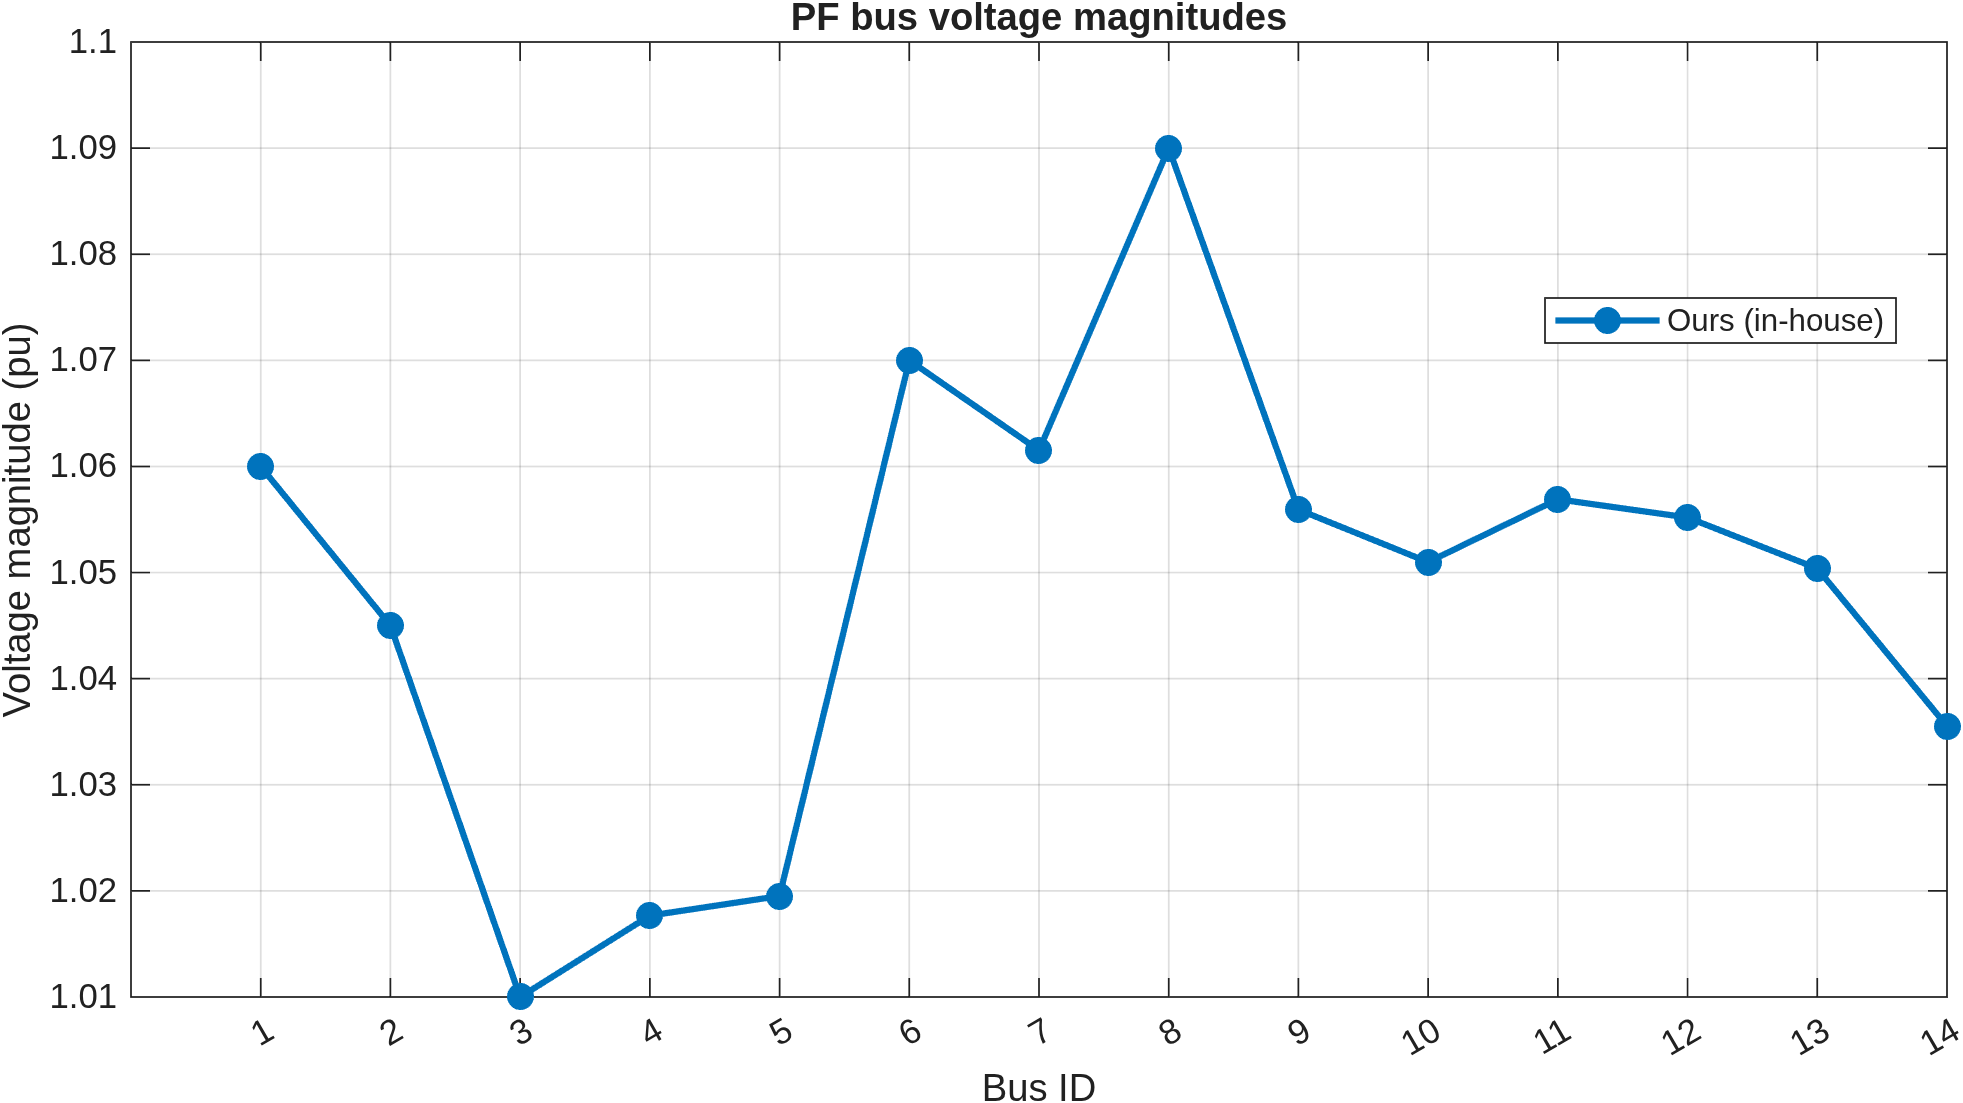
\includegraphics[width=0.95\textwidth]{figures/system_methods/ieee14_fig1_pf_voltage.png}
\caption{IEEE14 PF bus voltage magnitudes. Computed using PF-02--PF-18 from
\texttt{pfsolver.powerflow\_newton\_raphson}; generated by
\texttt{generate\_system\_methods\_report}; fresh at REPORT\_HEAD.}
\end{figure}

\begin{figure}[htbp]
\centering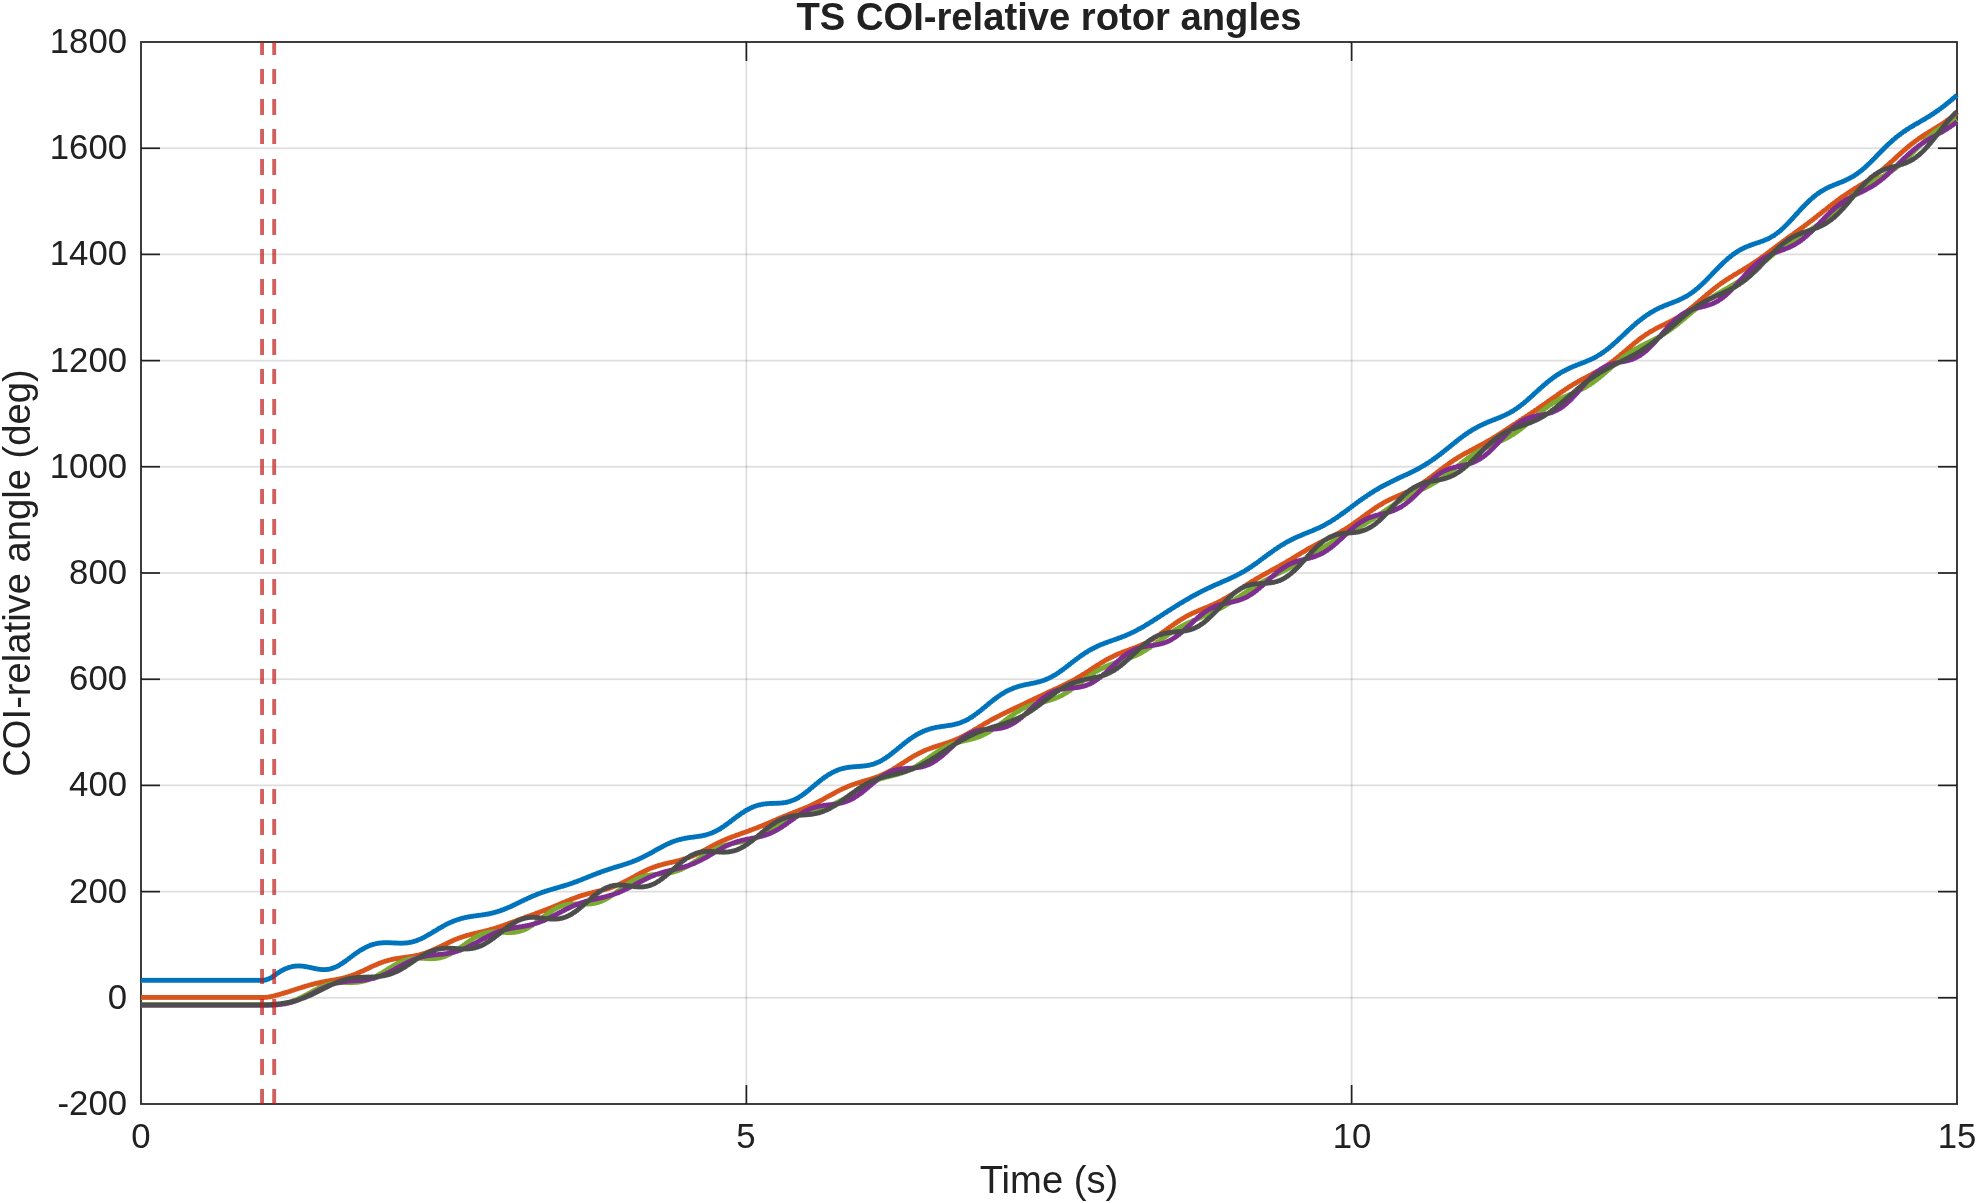
\includegraphics[width=0.95\textwidth]{figures/system_methods/ieee14_fig4_ts_coi_angle.png}
\caption{IEEE14 TS COI-relative rotor angles (Ours vs PSAT). Computed using
SG-C-01--12 + TS-F-01--12; fresh.}
\end{figure}

\begin{figure}[htbp]
\centering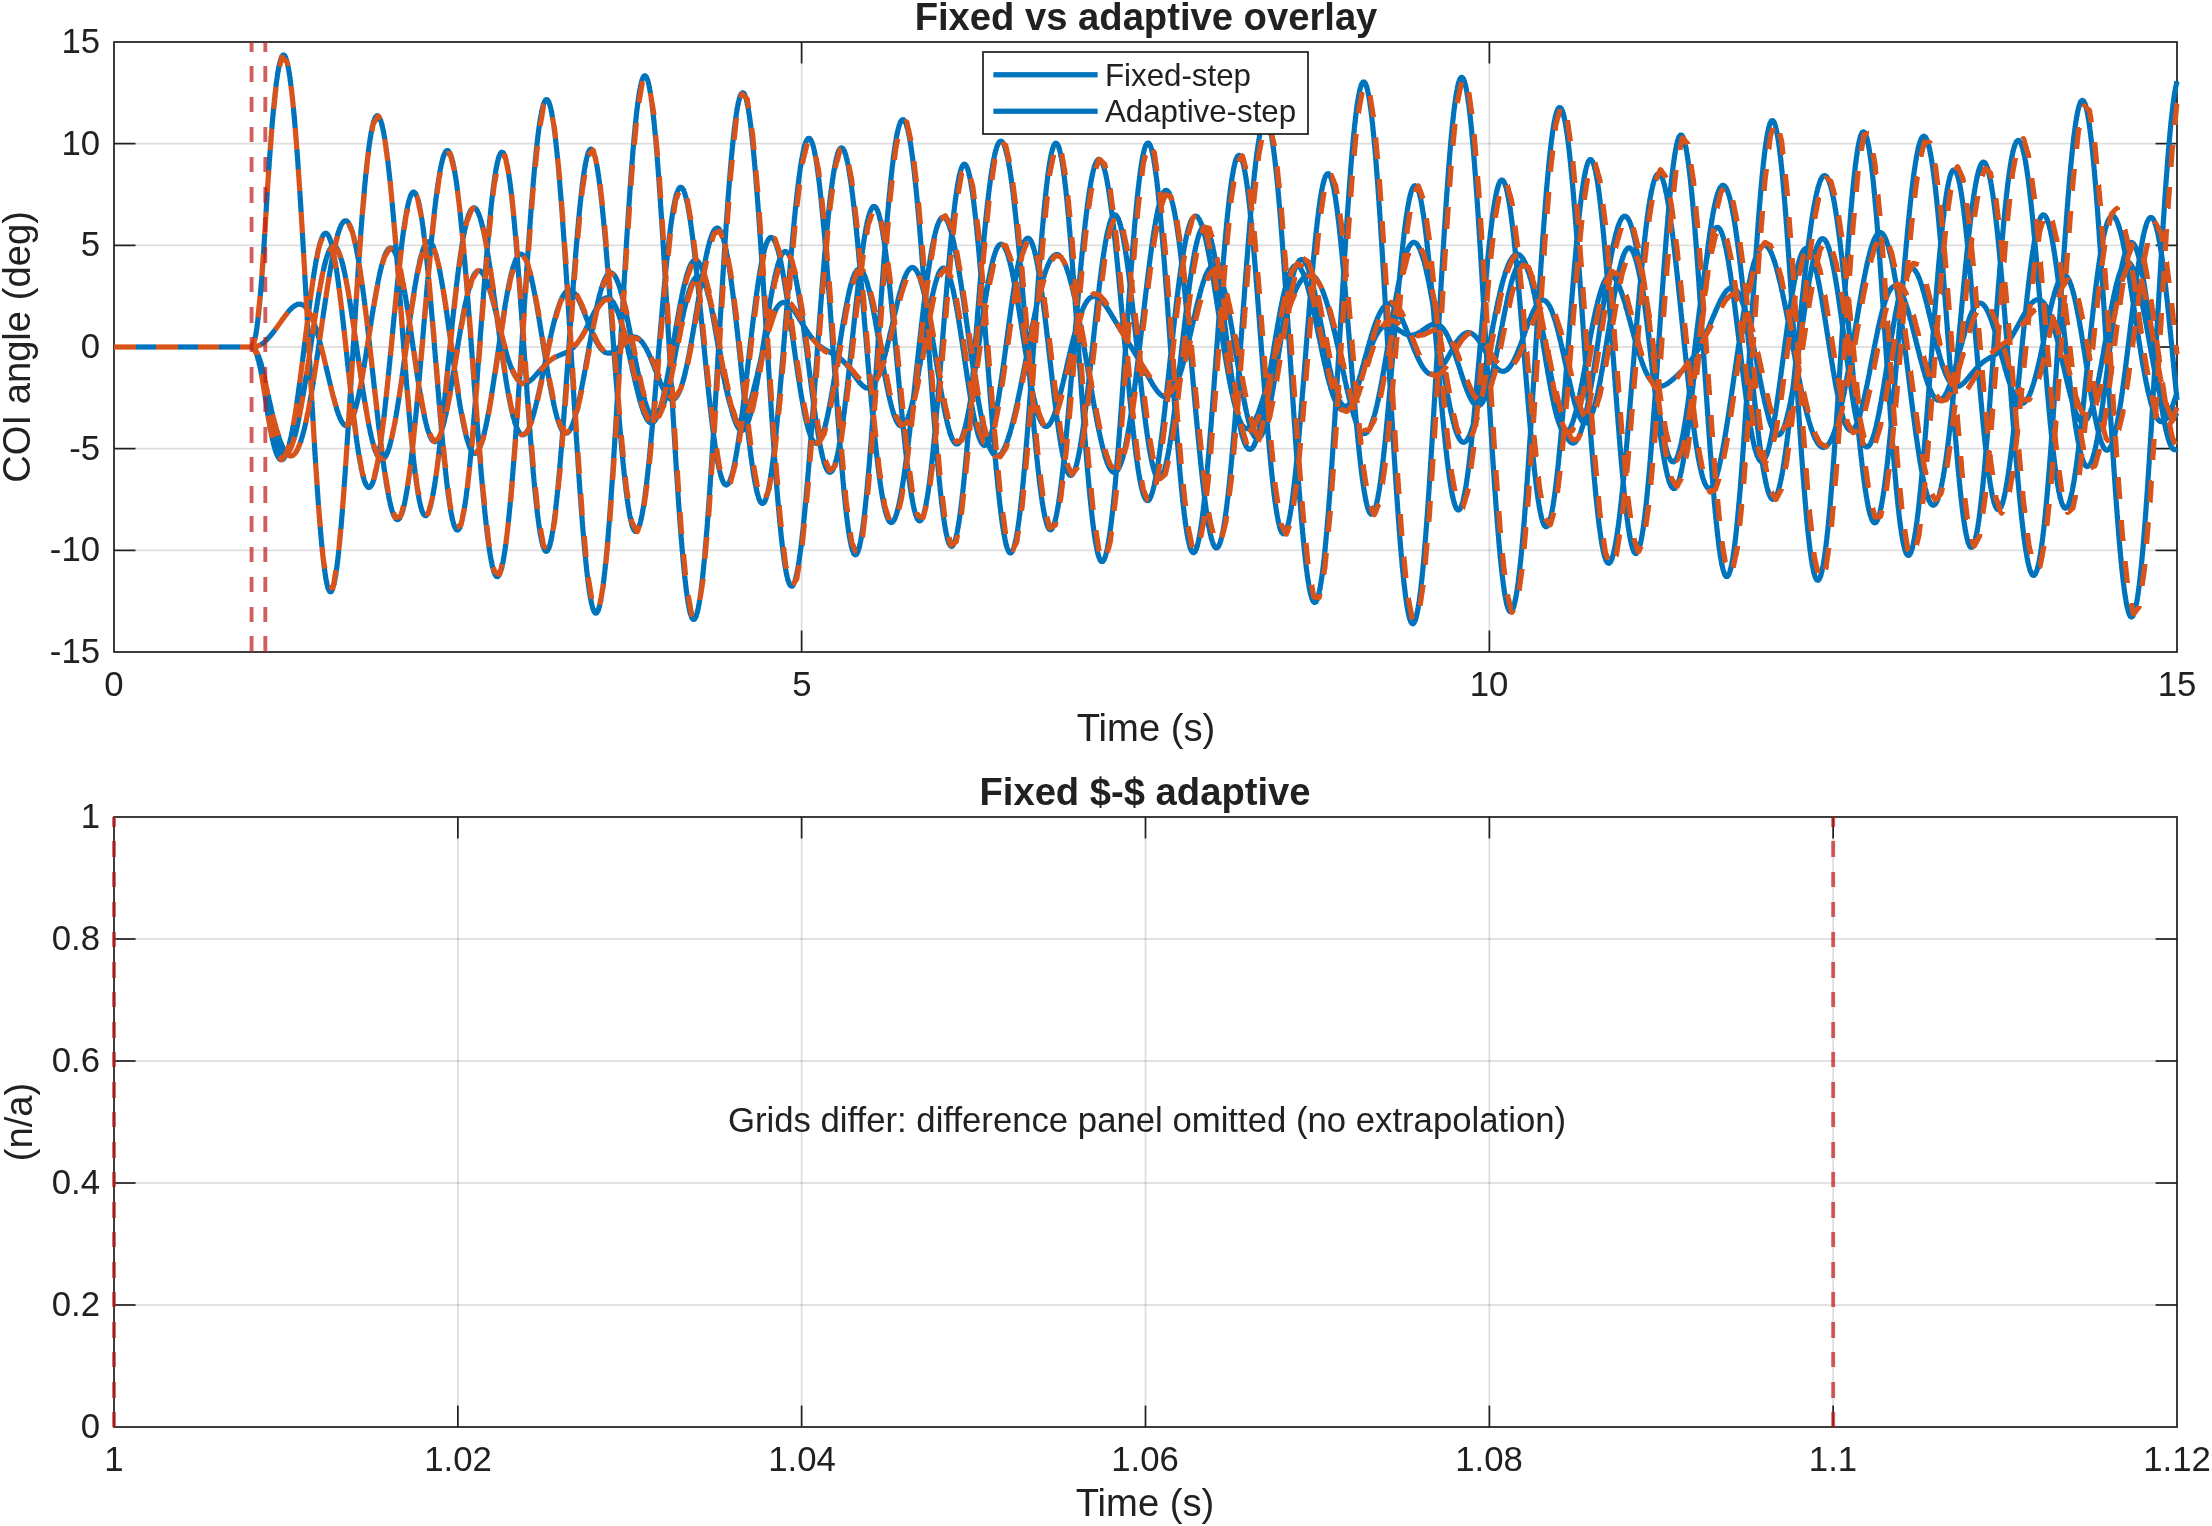
\includegraphics[width=0.95\textwidth]{figures/system_methods/ieee14_fig8_fixed_adaptive_overlay.png}
\caption{IEEE14 fixed vs adaptive TS overlay (classical model). Computed using
TS-A-01--16; adaptive is explicit, not default.}
\end{figure}

\section{IEEE RTS-24 study}

Ours vs PSAT (PGAz contract status: PGAz runs but TS discrepancy is
diagnostic only). Constant-impedance load conversion
$Y_{\mathrm{load}}=\overline{S_0}/|V_0|^2$ used at runtime
(\texttt{classical\_dae.m:51}); the case data itself uses constant-power
loads identical to the in-house PF.

% Generated by report_table_helpers. Do not edit by hand.
\begin{tabular}{lr}\toprule Quantity & Value \\ \midrule
converged &  \\
iterations & 5 \\
max\\_mismatch & 2.30926e-12 \\
P\\_total\\_gen\\_pu & 29.0125 \\
P\\_total\\_load\\_pu & 28.5 \\
P\\_loss\\_total\\_pu & 0.512464 \\
\bottomrule
\end{tabular}

% Generated by report_table_helpers. Do not edit by hand.
\begin{tabular}{lrrrr}\toprule Metric & Unit & Ours & PSAT & PGAz \\ \midrule
max\\_dCOI & deg & 0.0000e+00 & 6.7685e-03 & NaN \\
max\\_domega & pu & 0.0000e+00 & 4.6205e-06 & NaN \\
max\\_dPe & MW & 0.0000e+00 & 8.2709e-02 & NaN \\
max\\_dVbus & pu & 0.0000e+00 & 5.3538e-06 & NaN \\
\bottomrule
\end{tabular}

% Generated by report_table_helpers. Do not edit by hand.
\begin{tabular}{lr}\toprule Diagnostic & Value \\ \midrule
Accepted steps & 382 \\
Rejected steps & 5 \\
dt min & 1.0000e-02 s \\
dt max & 4.0000e-02 s \\
dt mean & 3.9267e-02 s \\
Error estimator max & 9.9967e-01 \\
Max $\Delta\delta_{COI}$ & 0.0000e+00 deg \\
Max pairwise angle diff & 0.0000e+00 deg \\
Max $\Delta\omega$ & 0.0000e+00 pu \\
Max $\Delta P_e$ & 0.0000e+00 pu \\
Max $\Delta V_{bus}$ & 0.0000e+00 pu \\
Readiness label & ADAPTIVE_DEFAULT_NOT_READY (explicit only) \\
\bottomrule
\end{tabular}


\section{Four-machine two-area study}

\subsection{Padiyar four-machine two-area}

\begin{tabular}{@{}lr@{}}\toprule Quantity & Value\\ \midrule
Converged & Yes\\
Iterations & 3\\
Maximum $|\Delta V|$ vs Table 9.2 & 4.927e-05 pu\\
Maximum $|\Delta \theta|$ vs Table 9.2 & 4.983e-05 deg\\
Total generation & 2821.72 MW\\
Total load & 2734.00 MW\\
Total loss & 87.72 MW\\
\bottomrule\end{tabular}

\begin{tabular}{rccrcl}\toprule
{No.} & {$\lambda_{book}$} & {$\lambda_{ours}$} & {$|\Delta\lambda|$} & {$\varepsilon_{\lambda}$} & {Mode}\\
{} & {(s$^{-1}$)} & {(s$^{-1}$)} & {(s$^{-1}$)} & {(\%)} & {}\\ \midrule
1 & $-39.9893$ & $-40.0225$ & 0.0332 & {0.08} & \\
2 & $-39.4922$ & $-39.5270$ & 0.0348 & {0.09} & \\
3 & $-24.5058 +20.6749j$ & $-24.5061 +20.6319j$ & 0.0430 & {0.13} & \\
4 & $-24.5058 -20.6749j$ & $-24.5061 -20.6319j$ & 0.0430 & {0.13} & \\
5 & $-25.0383 +11.9973j$ & $-25.0384 +11.9598j$ & 0.0375 & {0.13} & \\
6 & $-25.0383 -11.9973j$ & $-25.0384 -11.9598j$ & 0.0375 & {0.13} & \\
7 & $-11.5835$ & $-11.5566$ & 0.0269 & {0.23} & \\
8 & $-11.1735$ & $-11.1485$ & 0.0250 & {0.22} & \\
9 & $-0.7594 +7.2938j$ & $-0.7553 +7.3157j$ & 0.0223 & {0.30} & Swing 1\\
10 & $-0.7594 -7.2938j$ & $-0.7553 -7.3157j$ & 0.0223 & {0.30} & Swing 1\\
11 & $-0.7365 +6.6899j$ & $-0.7336 +6.7108j$ & 0.0211 & {0.31} & Swing 2\\
12 & $-0.7365 -6.6899j$ & $-0.7336 -6.7108j$ & 0.0211 & {0.31} & Swing 2\\
13 & $-0.0044 +4.4444j$ & $-0.0042 +4.4565j$ & 0.0121 & {0.27} & Inter-area\\
14 & $-0.0044 -4.4444j$ & $-0.0042 -4.4565j$ & 0.0121 & {0.27} & Inter-area\\
15 & $-4.5727$ & $-4.5701$ & 0.0026 & {0.06} & \\
16 & $-4.4802$ & $-4.4776$ & 0.0026 & {0.06} & \\
17 & $-4.1121$ & $-4.1095$ & 0.0026 & {0.06} & \\
18 & $0.0000 +0.0017j$ & $0.0000 +0.0000j$ & 0.0017 & {--} & \\
19 & $0.0000 -0.0017j$ & $0.0000 -0.0000j$ & 0.0017 & {--} & \\
20 & $-4.2449$ & $-4.2423$ & 0.0026 & {0.06} & \\
\bottomrule\end{tabular}

\begin{tabular}{llrr}\toprule {Metric} & {Unit} & {AVR} & {Manual excitation}\\ \midrule
Initial DAE residual & pu & 9.215e-13 & 5.684e-14\\
Non-converged steps & steps & 0 & 0\\
Maximum corrector residual & pu & 7.676e-09 & 5.107e-10\\
Minimum bus voltage & pu & 0.9244 & 0.9184\\
Maximum speed deviation & pu & 4.397e-04 & 8.002e-04\\
\bottomrule\end{tabular}


\begin{figure}[htbp]
\centering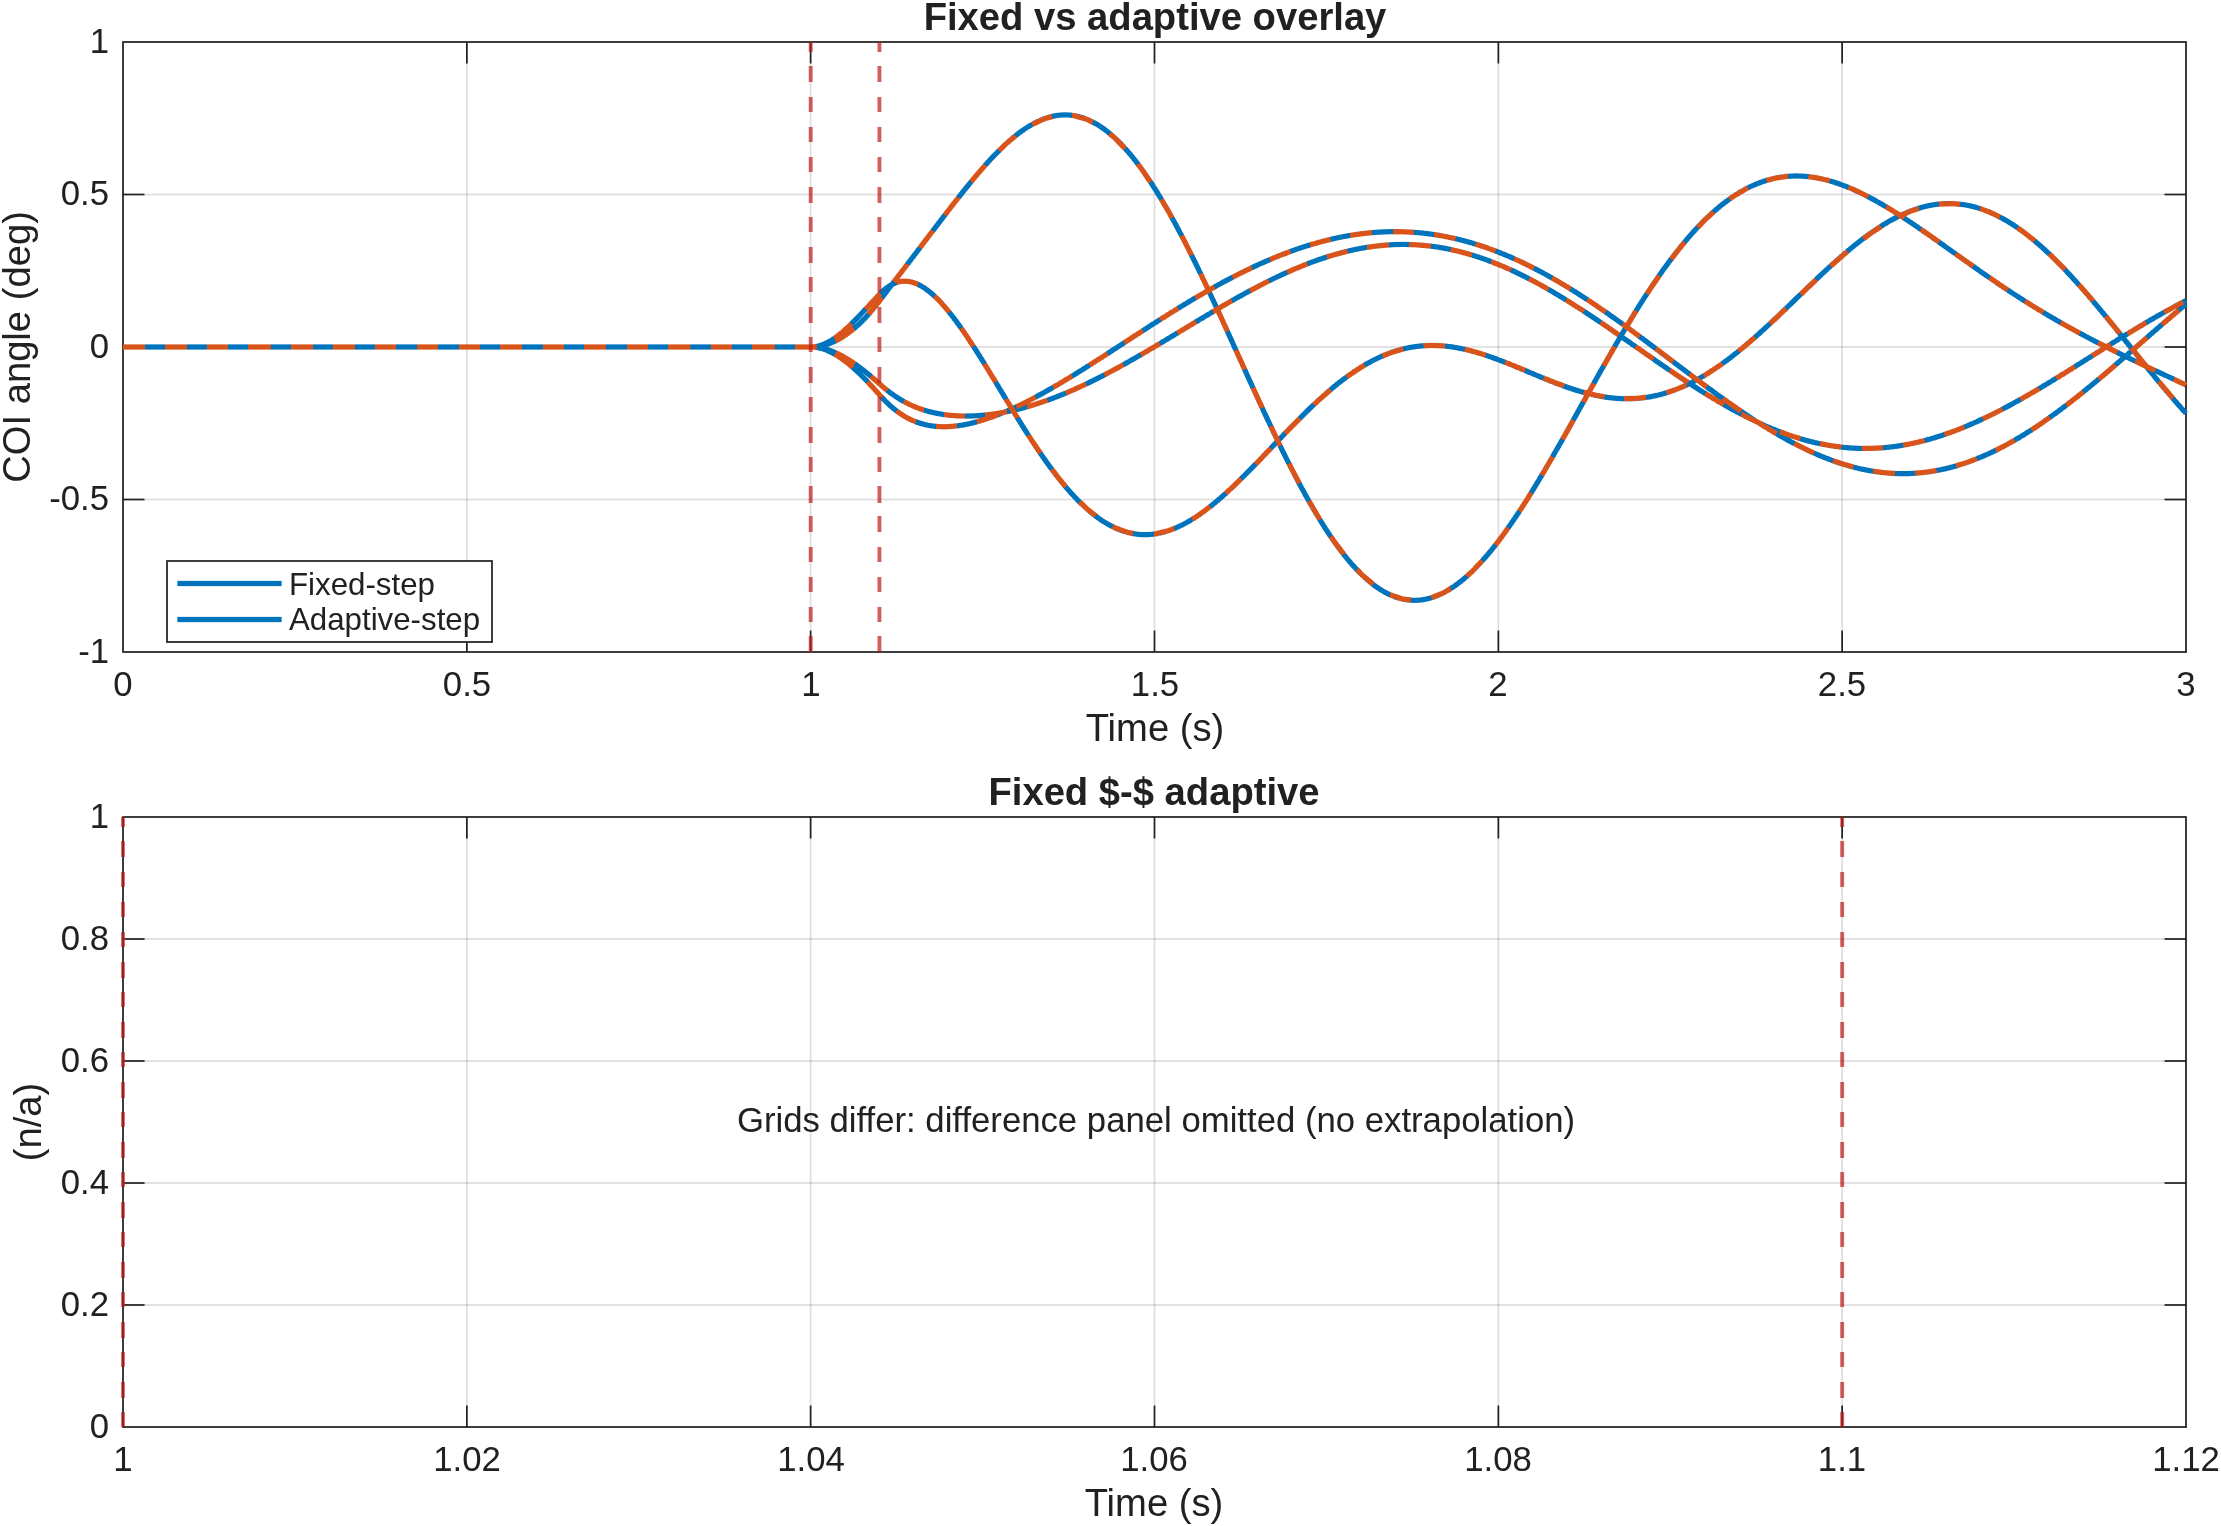
\includegraphics[width=0.95\textwidth]{figures/padiyar_two_area/padiyar_fixed_adaptive_overlay.png}
\caption{Padiyar 4M2A fixed vs adaptive TS overlay (model-1.1 AVR). Computed
using SG-P-01--06 + TS-A-01--16; fresh.}
\end{figure}

\subsection{Kundur four-machine two-area}

Not used in this report. Legacy calibrated GENTPJ and primitive-flux paths are
excluded from acceptance results per AGENTS.md.

\section{Cross-case synthesis}

% Generated by report_table_helpers. Do not edit by hand.
\begin{longtable}{lrrrrr l}\toprule
Case & PF max mismatch & PF ext. err & Dominant mode & TS bounded & Fixed/Adaptive diff & Status \\ \midrule
case_padiyar_two_area_4m_avr & NaN & NaN & pending & pending & NaN & pending \\
\bottomrule
\end{longtable}


No unqualified PASS is declared; per-case metrics and limitations are reported.

\section{Limitations and readiness}

\begin{itemize}[leftmargin=1.5em]
\item IEEE14 SG dynamic data is ASSUMED\_DIAGNOSTIC (MATPOWER network/PF only).
\item Adaptive timestep is explicit, not default
      (\texttt{ADAPTIVE\_DEFAULT\_SWITCH\_READY=NOT\_READY}).
\item Tolerance-selection evidence for the adaptive controller is structural
      (execution + analytic LTE test), not a held-out prospective validation.
\item PGAz is a secondary diagnostic only; PGAz mismatches are reported
      honestly and do not fail the gate.
\item IBR production integration: \texttt{IBR\_PRODUCTION\_INTEGRATION\_READY=NOT\_STARTED}.
\item Kundur 4M2A not reported (legacy calibrated paths excluded).
\item Hairer section/page for the Richardson estimator is unverified on this
      host; the estimator is PROJECT\_DERIVED (proven by analytic test).
\end{itemize}

\section{Reproduction instructions}

\begin{lstlisting}
restoredefaultpath;
cd('<report worktree>');
pf_init_paths;
generate_system_methods_report;
\end{lstlisting}

LaTeX build:
\begin{lstlisting}
cd docs/source
pdflatex report_system_methods_update
pdflatex report_system_methods_update
\end{lstlisting}

\paragraph{Equation provenance.} The full equation provenance register, symbol
dictionary, source-input provenance, code mapping, and source gaps are
generated into \texttt{figures/system\_methods/} by
\texttt{equation\_register\_export}. The fail-closed audit
(\texttt{equation\_audit}) asserts \texttt{DOCUMENTATION\_EQUATION\_PROVENANCE\_READY=READY}.

% Generated by equation_register_export. Do not edit by hand.
\section*{Equation source gaps}

\begin{tabular}{lll}\toprule Equation ID & Rule & Detail \\\midrule
\bottomrule
\end{tabular}

\paragraph{Audit status.}
\begin{tabular}{ll}\toprule Gate & Status \\\midrule
EQUATION\_REGISTER\_COMPLETE & READY \\
EQUATION\_SOURCE\_COVERAGE & READY \\
DIMENSIONAL\_AUDIT & READY \\
CONVENTION\_AUDIT & READY \\
CODE\_EQUATION\_MATCH & READY \\
PROJECT\_DERIVED\_PREMISES & READY \\
RESULT\_PROVENANCE\_COMPLETE & PENDING \\
DOCUMENTATION\_EQUATION\_PROVENANCE\_READY & READY \\
\bottomrule
\end{tabular}


\end{document}
